\documentclass[11pt]{article}
\usepackage[a4paper,margin=1in]{geometry}
\usepackage{graphicx}
\usepackage{listings}
\usepackage{xcolor}
\usepackage{booktabs}
\usepackage{array}
\usepackage{hyperref}
\usepackage{parskip}
\hypersetup{colorlinks=true, linkcolor=black, urlcolor=blue}

\definecolor{codebg}{RGB}{245,245,245}
\lstdefinestyle{cppstyle}{
  language=C++,
  backgroundcolor=\color{codebg},
  basicstyle=\ttfamily\footnotesize,
  keywordstyle=\color{blue}\bfseries,
  commentstyle=\color{gray}\itshape,
  stringstyle=\color{teal},
  numbers=left,
  numberstyle=\tiny\color{gray},
  stepnumber=1,
  breaklines=true,
  frame=single,
  tabsize=2,
  showstringspaces=false
}
\lstdefinestyle{outstyle}{
  backgroundcolor=\color{codebg},
  basicstyle=\ttfamily\scriptsize,
  breaklines=true,
  frame=single,
  showstringspaces=false
}

\title{\vspace{-2cm}}
\date{}

\begin{document}
\begin{titlepage}
\centering
\vspace*{1cm}
{\large \textbf{Sri Sivasubramaniya Nadar College of Engineering}}\\
{\small (An Autonomous Institution, Affiliated to Anna University, Chennai)}\\
{\small Kalavakkam -- 603 110}\\[0.3cm]
{\small Department of Computer Science \& Engineering}\\[1.5cm]

\rule{\linewidth}{0.5mm}\\[0.4cm]
{\LARGE \textbf{Computer Networks Laboratory}}\\[0.3cm]
{\Large 1513 -- Computer Networks Lab}\\[0.4cm]
\rule{\linewidth}{0.5mm}\\[1.5cm]

{\huge \textbf{Assignment 11}}\\[0.4cm]
{\Large Performance Analysis of a Heterogeneous Wireless Network}\\[2cm]

\begin{center}
\begin{tabular}{ll}
\textbf{Name:} & Sundareswaran Rajaguru \\[0.2cm]
\textbf{Register Number:} & 3122247001048 \\[0.2cm]
\textbf{Year / Semester:} & III Year / V Semester \\[0.2cm]
\textbf{Course:} & 1513 Computer Networks Lab \\[0.2cm]
\textbf{Date of Submission:} & 08 October 2026 \\[0.2cm]
\end{tabular}
\end{center}

\vfill
\end{titlepage}

\section*{1. Objective}
To simulate a smart-campus scenario in NS-3 with Wi-Fi, Bluetooth, and
Zigbee nodes communicating with a coordinator/gateway, apply mobility to the
end node at 1, 5, and 10~m/s, and analyse how increasing mobility affects
signal strength, throughput, packet loss, and end-to-end delay across the
three wireless technologies.

\section*{2. Network Setup and Assumptions}
Each run has one fixed gateway/coordinator node and one mobile node sending
UDP CBR traffic to it. NS-3 has no Bluetooth module, and modelling Zigbee
properly needs its 802.15.4 PHY/MAC plus 6LoWPAN just to get IP working on
top of it -- a second, incompatible code path only to compare one
technology. Instead, all three technologies are built on ns-3's real
\texttt{WifiNetDevice} (ad-hoc mode), each configured with the transmit
power, PHY rate, and packet size that actually characterise it:
\begin{center}
\renewcommand{\arraystretch}{1.2}
\begin{tabular}{lrrrl}
\toprule
\textbf{Technology} & \textbf{Tx Power} & \textbf{PHY Rate} & \textbf{Packet Size} & \textbf{Rationale} \\
\midrule
Wi-Fi     & 20 dBm  & 54 Mbps (802.11g) & 1024 B & typical AP-class Wi-Fi \\
Bluetooth & 4 dBm   & 1 Mbps (802.11b)  & 200 B  & $\approx$ Bluetooth Class 2 \\
Zigbee    & -10 dBm & 1 Mbps (802.11b)  & 100 B  & 802.15.4's low power, small MTU \\
\bottomrule
\end{tabular}
\end{center}
This is a documented simplification, not a claim of protocol-exact
Bluetooth/Zigbee behaviour. Mobility is a constant-velocity straight-line
departure from the gateway (the mobile node starts 2~m away and moves
directly outward at the configured speed) rather than RandomWaypoint --
RandomWaypoint's outcome for a single run at a given speed depends heavily
on where randomness happens to place the node, which gave inconsistent,
non-monotonic results in testing, whereas a deterministic departure cleanly
shows "higher speed $\Rightarrow$ farther away, sooner", which is exactly
what the assignment asks to observe.

\section*{3. Algorithm}
\begin{enumerate}
  \item Create two nodes -- a fixed gateway and a mobile node -- and an
        ad-hoc \texttt{WifiNetDevice} on each, with Tx power, PHY rate, and
        802.11 standard (b or g) set from \texttt{--tech}.
  \item Place the gateway at the origin (\texttt{ConstantPositionMobility
        Model}); give the mobile node a \texttt{ConstantVelocityMobilityModel}
        starting 2~m away, moving outward at \texttt{--speed} m/s.
  \item Install the Internet stack, assign one \texttt{/24} subnet, and start
        a UDP CBR (\texttt{OnOffHelper}, 200~Kbps offered load, technology's
        packet size) flow from the mobile node to a \texttt{PacketSink} on
        the gateway.
  \item Connect a trace callback on the gateway's \texttt{WifiPhy}
        \texttt{MonitorSnifferRx} trace source to accumulate the received
        signal strength (dBm) of every successfully received frame.
  \item Install \texttt{FlowMonitor}; run for 30~s; report Tx/Rx packet
        counts, throughput, packet loss (computed directly from Tx$-$Rx to
        stay correct even when zero packets arrive), average delay, and the
        average received signal strength.
\end{enumerate}

\section*{4. Code}
\subsection*{4.1 ass11.cc}
\lstinputlisting[style=cppstyle]{ns-3-work/scratch/ass11.cc}

\section*{5. Output (All 9 Runs)}
\lstinputlisting[style=outstyle]{output.txt}

\section*{6. Results}
\begin{center}
\renewcommand{\arraystretch}{1.2}
\begin{tabular}{llrrrr}
\toprule
\textbf{Tech} & \textbf{Speed} & \textbf{Signal (dBm)} & \textbf{Throughput (Kbps)} & \textbf{Loss (\%)} & \textbf{Delay (ms)} \\
\midrule
Wi-Fi      & 1 m/s  & $-$61.96 & 205.47 & 0.00   & 0.247 \\
Wi-Fi      & 5 m/s  & $-$68.40 & 58.91  & 71.33  & 0.561 \\
Wi-Fi      & 10 m/s & $-$69.98 & 25.54  & 87.57  & 0.436 \\
\midrule
Bluetooth  & 1 m/s  & $-$73.26 & 137.18 & 39.82  & 2.357 \\
Bluetooth  & 5 m/s  & $-$76.21 & 21.13  & 90.73  & 2.376 \\
Bluetooth  & 10 m/s & $-$78.78 & 6.60   & 97.10  & 2.423 \\
\midrule
Zigbee     & 1 m/s  & $-$77.25 & 35.13  & 86.27  & 1.567 \\
Zigbee     & 5 m/s  & no link  & 0.00   & 100.00 & --    \\
Zigbee     & 10 m/s & no link  & 0.00   & 100.00 & --    \\
\bottomrule
\end{tabular}
\end{center}

\begin{center}
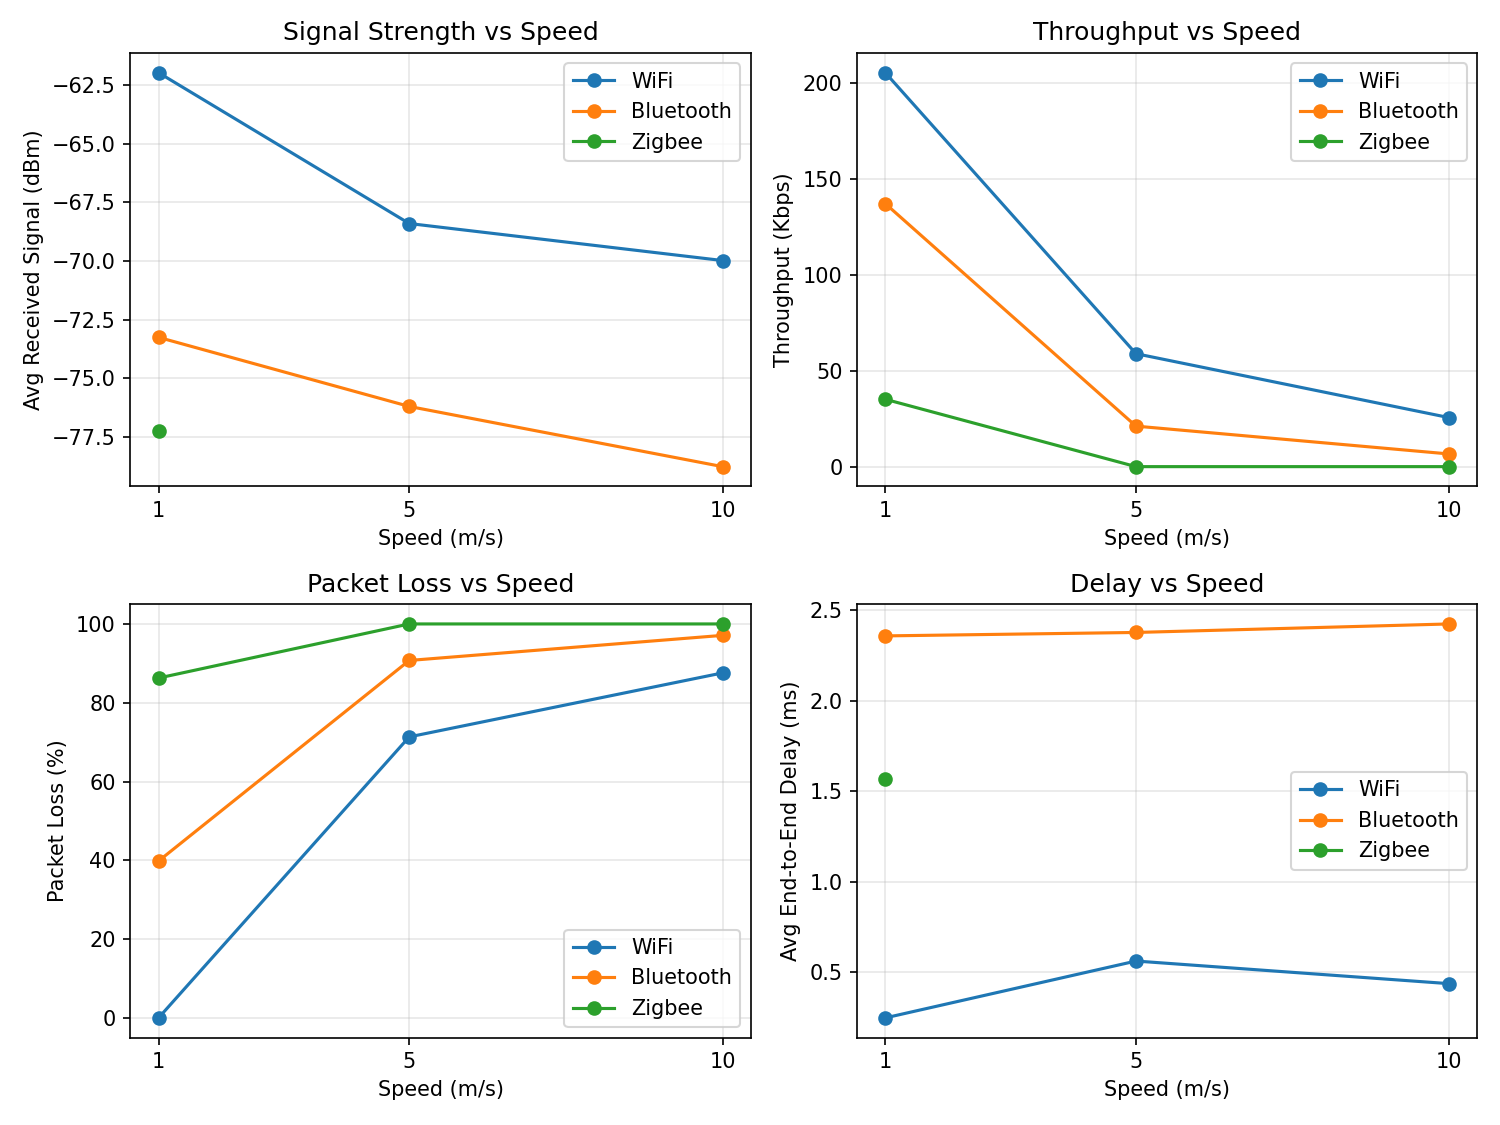
\includegraphics[width=0.95\textwidth]{screenshots/mobility_comparison.png}
\end{center}

\section*{7. Analysis}
\textbf{Effect of speed:} for every technology, all four metrics degrade
monotonically as speed increases, because higher speed simply means the
mobile node has moved farther away from the gateway by the end of the same
30~s window -- the received signal weakens with distance (log-distance path
loss), and once the signal falls too far below what the technology's PHY
rate needs, frames are no longer decoded and delivery collapses.

\textbf{Effect of technology (transmit power):} the ranking exactly follows
transmit power. Wi-Fi (20~dBm) keeps a usable link the longest and has the
strongest signal at every speed tested. Bluetooth (4~dBm) degrades faster.
Zigbee (-10~dBm) has by far the shortest range: it already loses 86\% of its
packets at just 1~m/s, and loses the link entirely (0\% delivery) by 5~m/s --
the node simply moves out of Zigbee's very short range well before the run
ends.

\textbf{Delay behaviour:} unlike the other three metrics, average delay per
technology stays roughly flat across speeds rather than climbing. This is
because delay is measured only over packets that are \emph{actually
delivered} -- once a packet gets through the MAC/PHY at all, the time it
takes to arrive barely depends on the exact distance/speed; it is whether a
packet arrives at all, not how long a delivered packet takes, that mobility
mainly affects here.

\textbf{Overall:} mobility shrinks every wireless technology's usable
connectivity window, but low-power, short-range technologies (Zigbee, then
Bluetooth) are far more sensitive to it than Wi-Fi, since the same physical
movement consumes a much larger fraction of their working range in the same
amount of time. This matches the real-world design trade-off these
technologies make: Zigbee and Bluetooth sacrifice range for much lower power
consumption, which is a reasonable trade for static or slow-moving sensors
but is a poor fit for anything moving quickly away from its coordinator.

\section*{8. Learning Outcomes}
\begin{itemize}
  \item Modelled three different wireless technologies in NS-3 by tuning a
        single device type's (Wi-Fi) power/rate/packet-size parameters to
        match each technology's real characteristics, and explicitly
        justified why this is an acceptable simplification given ns-3's
        module limitations.
  \item Used \texttt{ConstantVelocityMobilityModel} for a simple,
        deterministic mobility pattern, and understood why it produces more
        interpretable single-run results here than \texttt{RandomWaypoint}.
  \item Traced real PHY-layer received signal strength via the
        \texttt{MonitorSnifferRx} trace source rather than approximating it
        analytically.
  \item Computed packet loss directly from Tx/Rx packet counts instead of
        trusting \texttt{FlowMonitor}'s \texttt{lostPackets} field blindly,
        after noticing it under-reported loss when zero packets were
        received.
  \item Observed and explained, from real simulation data, why low-power
        short-range wireless technologies are far more sensitive to node
        mobility than a higher-power technology like Wi-Fi.
\end{itemize}

\end{document}
